\providecommand{\myrootdir}{..}
\documentclass[\myrootdir/main.tex]{subfiles}

\begin{document}

\chapter{Technique Comparison Study}
\label{evaluation}
running evaluation to compare the different techniques

\section{Study Design}
\includegraphics[page=6, width=\textwidth, trim={0.5cm 0.5cm 0.5cm 0.5cm}, clip]{img/flow-of-research.pdf}
\todo{run!}

taking The Failing Build Log Data Set - run 3(4 with random) techniques with increasing example count - measuring xyz - justify choices like running chronologically / testing on 1 example / no k-fold validation - how are keywords for the search selected?

\section{Study Results}
\todo{accuracy (or so) of extractions with growing example number // overall averages \& detailed look on special cases //}

\section{Resulting Recommending Scheme}
\todo{draw decision tree}

interpret results - when should PROSE be used? - when should text similarity be used? - when should keyword search be used? - answer RQ about PROSE \& other techniques

\end{document}
